\chapter{Segnali elementari}
\section{A tempo continuo}

\subsubsection{Segnali sinusoidali o fasori}

$ v(t)= Acos(wt+ \phi)$ con $t \in \mathbb{R}$.\\
Chiameremo: ampiezza $ A>0$, fase $ \phi $ (e se $ \phi > 0$ ho il segnale traslato a sinistra) , codominio $ [-A...A]$, periodo $ T = \frac{2 \pi}{w} $, pulsazione $w=\frac{2 \pi}{T} $ e frequenza $ f = \frac{1}{T}$ (NB: più grande è $T $ più piccola è f).\\
NB: $ w = 2 \pi f $ \\
NB: Come visto nell'Introduzione posso vedere il coseno come $  cosw = \frac{e^{jw} + e^{-jw}}{2}  $, quindi in questo caso $ cos(wt + \phi) = \frac{e^{jw+ \phi} + e^{-jw + \phi}}{2} $.\\

\subsubsection{Segnali sinusoidali modulati esponenzialmente}

$ v(t)= A e^{ \sigma t} cos(wt+ \phi)$ con $A>0$.\\
NB: In questo caso $T = \frac{2 \pi}{w} $ non è il periodo!\\

\begin{equation*}
v(t)=
\begin{cases} 
 \mbox{Converge, se } \sigma < 0 \rightarrow \mbox{ Il sistema è stabile }\\ 
 \mbox{Diverge, se } \sigma > 0 \rightarrow \mbox{ Il sistema è instabile}
\end{cases} 
\end{equation*}
Cioè $  \lim_{t \to \infty} v(t)=0$, solo se $ \sigma <0$.

\begin{figure}[h]
	\centering
	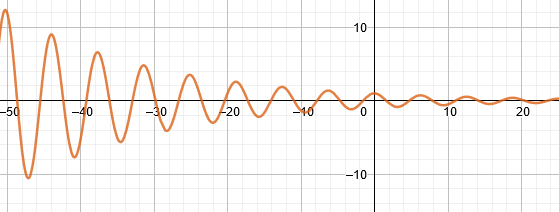
\includegraphics[scale=0.75]{immagini/segnSinNeg}
	\caption{ Andamento del segnale con $ \sigma <0$ }
	\label{fig: segnSinNeg}
\end{figure}

\pagebreak

\begin{figure}[h]
	\centering
	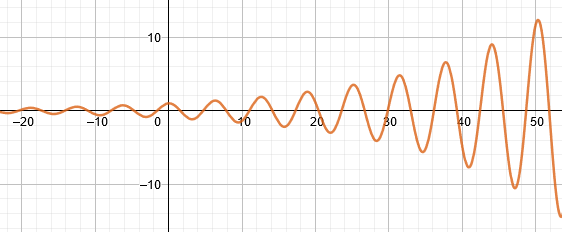
\includegraphics[scale=0.75]{immagini/segnSinPos}
	\caption{ Andamento del segnale con $ \sigma >0$ }
	\label{fig: segnSinPos}
\end{figure}

Come visto per il precedente segnale posso scrivere il coseno come $  cosw = \frac{e^{jw} + e^{-jw}}{2}  $.\\
In questo caso posso scrivere il segnale come:\\
$ v(t)= \frac{A}{2} e^{ \sigma t} e^{j(wt+ \phi)} + \frac{A}{2} e^{ \sigma t} e^{-j(wt+ \phi)}$\\
$= \frac{A}{2} e^{ \sigma t} e^{ jwt} e^{j \phi} + \frac{A}{2} e^{ \sigma t} e^{ -jwt} e^{-j \phi}$\\
$= \frac{A}{2} e^{j \phi} e^{( \sigma + jw) t} + \frac{A}{2} e^{-j \phi} e^{( \sigma - jw) t}$\\
Con $ s = \sigma + jw $ e $ \bar{s} = \sigma - jw $ posso scrivere che:\\
$= \frac{A}{2} e^{j \phi} e^{st} + \frac{A}{2} e^{-j \phi} e^{\bar{s} t}$\\
Cioè il segnale è la combinazione lineare di esponenziali complesse di cui una è il complesso conugato dell'altra.\\
 

\subsection{Funzioni generalizzate o distribuzioni}

Con distribuzioni intendiamo limiti di successioni di funzioni.\\

\subsubsection{Gradino unitario}
	
	\begin{equation*}
	\delta_{-1}(t)=
	\begin{cases} 
	1, \mbox{ se } t \geq 0\\ 
	0, \mbox{ se } t < 0
	\end{cases} 
	\end{equation*}
	
	\begin{figure}[h]
		\centering
		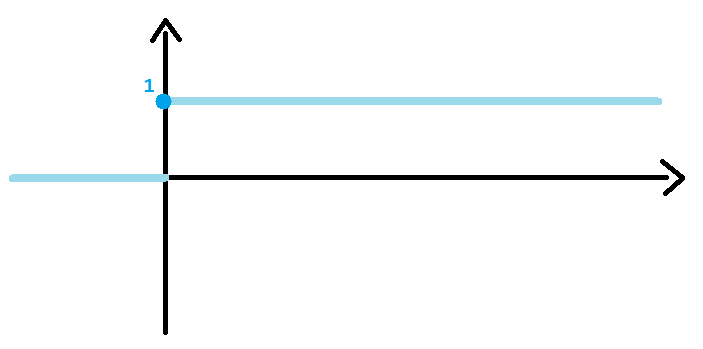
\includegraphics[scale=0.5]{immagini/gradinoContinuo}
		\caption{ Gradino unitario}
		\label{fig: gradinoContinuo}
	\end{figure}
	
	Proviamo ora a traslarla, con $ t_0 > 0$.\\
	
	Per avere un segnale in ritardo, dovrò traslare a destra e quindi sottraggo $t_0$.\\
	
	\begin{equation*}
	\delta_{-1}(t - t_0 )=
	\begin{cases} 
	1, \mbox{ se } t \geq t_0\\ 
	0, \mbox{ se } t < t_0
	\end{cases} 
	\end{equation*}
	
	\begin{figure}[h]
		\centering
		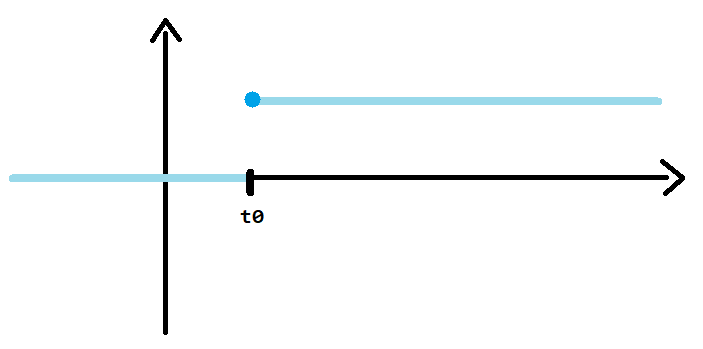
\includegraphics[scale=0.5]{immagini/gradinoContinuoMeno}
		\caption{ Gradino unitario $ \delta_{-1}(t - t_0 ) $ }
		\label{fig: gradinoContinuoMeno}
	\end{figure}
	
	Per avere un segnale in anticipo, dovrò traslare a sinistra e quindi sommo $t_0$.\\
	
	\begin{equation*}
	\delta_{-1}(t + t_0)=
	\begin{cases} 
	1, \mbox{ se } t \geq -t_0\\ 
	0, \mbox{ se } t < -t_0
	\end{cases} 
	\end{equation*}
	
	\begin{figure}[h]
		\centering
		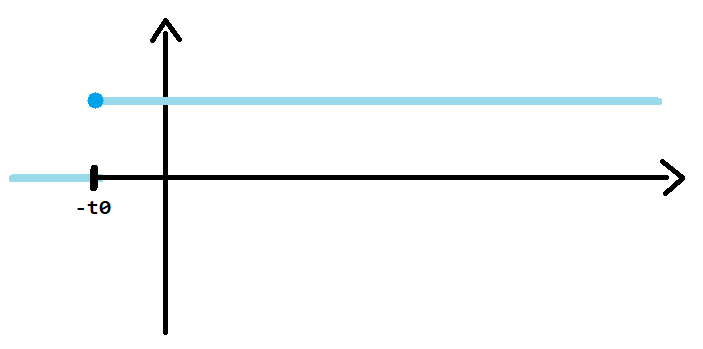
\includegraphics[scale=0.5]{immagini/gradinoContinuoPiu}
		\caption{ Gradino unitario $ \delta_{-1}(t + t_0 ) $ }
		\label{fig: gradinoContinuoPiu}
	\end{figure}
	
\pagebreak
	
	\textbf{COMANDO MATLAB:}\\
	
	\begin{figure}[h]
		\centering
		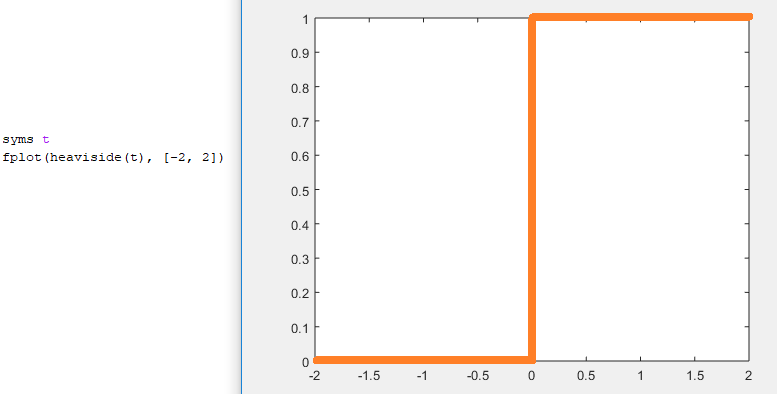
\includegraphics[scale=0.75]{immagini/comando2}
		\caption{ Il comando syms crea una variabile t, heaviside è la funzione per il gradino, fplot "plotta" cioè fa il grafico fra [-2...2]  }
		\label{fig: comando2}
	\end{figure}
	
	NB: da notare come la funzione gradino non è continua ma riusciremo comunque a derivarla.\\

\subsubsection{Funzione rettangolare di ampiezza e durata unitaria}
	
	\begin{equation*}
	\varPi(t)=
	\begin{cases} 
	1, \mbox{ se } -\frac{1}{2} \leq t \leq \frac{1}{2}\\ 
	0, \mbox{ altrimenti }
	\end{cases} 
	\end{equation*}
	
	\begin{figure}[h]
		\centering
		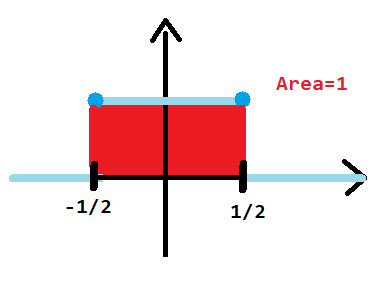
\includegraphics[scale=0.5]{immagini/rettangolo}
		\caption{ Funzione rettangolare di ampiezza e durata unitaria $ \varPi(t) $ }
		\label{fig: rettangolo}
	\end{figure}
	
	NB: è una combinazione lineare di due gradini:\\
	$ \varPi(t)= \delta_{-1}(t + \frac{1}{2}) - \delta_{-1}(t-\frac{1}{2}) $\\
	
	In generale il segnale sarà $ A \varPi( \frac{t-t_0}{T}) $, che mi dà una finestra di ampiezza A, durata T e centrata in $t_0$.\\
	
	\begin{equation*}
	A \varPi( \frac{t-t_0}{T})=
	\begin{cases} 
	A, \mbox{ se } -\frac{1}{2} \leq \frac{t-t_0}{T} \leq \frac{1}{2} \rightarrow -\frac{T}{2}+t_0 \leq t \leq \frac{T}{2}+ t_0 \\ 
	0, \mbox{ altrimenti }
	\end{cases} 
	\end{equation*}
	
	\begin{figure}[h]
		\centering
		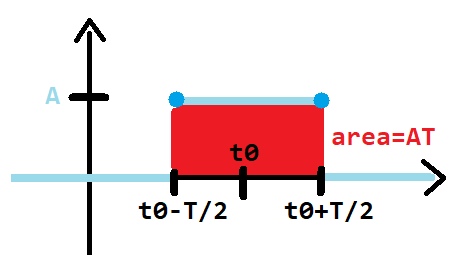
\includegraphics[scale=0.5]{immagini/rettangoloGenerale}
		\caption{ Funzione rettangolare in generale $ A \varPi( \frac{t-t_0}{T}) $ }
		\label{fig: rettangoloGenerale}
	\end{figure}


\subsubsection{Lambda: impulso triangolare di ampiezza e area unitaria}
	
	\begin{equation*}
	\varLambda(t)=
	\begin{cases} 
	0, \mbox{ se } t \leq -1\\ 
	1-|t|, \mbox{ se } -1 \leq t \leq 1\\ 
	0, \mbox{ se }  t > 1
	\end{cases} 
	\end{equation*}
	
	\begin{figure}[h]
		\centering
		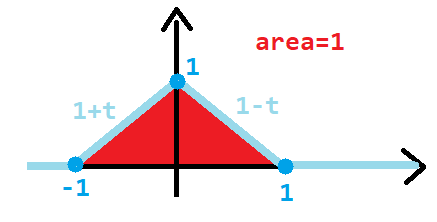
\includegraphics[scale=0.5]{immagini/lambda}
		\caption{ Funzione lambda $ \varLambda(t) $ }
		\label{fig: lambda}
	\end{figure}
	
	In generale il segnale sarà $ A \varLambda(t-t_0) $.\\
	
	\begin{equation*}
	A \varLambda( \frac{t-t_0}{T})=
	\begin{cases} 
	0, \mbox{ se } t \leq t_0-T\\ 
	\dfrac{A}{T}(|t|-t_0+T), \mbox{ se } t_0-T \leq t \leq t_0+T\\ 
	0, \mbox{ se }  t > t_0+T
	\end{cases} 
	\end{equation*}
	
	\begin{figure}[h]
		\centering
		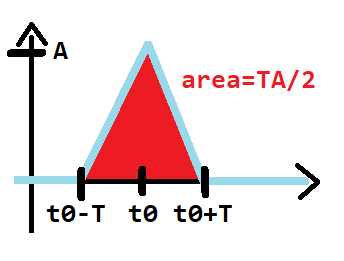
\includegraphics[scale=0.5]{immagini/lambdaGenerale}
		\caption{ Funzione lambda in generale $ A \varLambda( \frac{t-t_0}{T}) $ }
		\label{fig: lambdaGenerale}
	\end{figure}

\pagebreak

\subsubsection{Rampa unitaria}

	\begin{equation*}
	\delta_{-2}(t)=
	\begin{cases} 
	t, \mbox{ se } t \geq 0\\ 
	0, \mbox{ altrimenti }
	\end{cases} 
	\end{equation*}
	
	\begin{figure}[h]
		\centering
		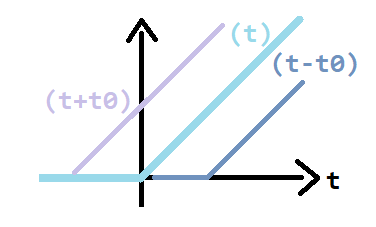
\includegraphics[scale=0.5]{immagini/rampaContinua}
		\caption{ Funzione rampa unitaria $\delta_{-2}(t) $ }
		\label{fig: rampaContinua}
	\end{figure}

\subsubsection{Riassunto: colleghiamo le distribuzioni}

	Notiamo che $ \delta_{-2}(t) = \int_{ -\infty}^{t} \delta_{-1}(\tau)  \, d \tau  $, sappiamo anche che per $ \tau <0 $ abbiamo $ \delta_{-1}(\tau) = 0 $ quindi $ \int_{ 0}^{t} \delta_{-1}(\tau)  \, d \tau $. Da 0 a t, ho $ \delta_{-1}(\tau) = 1 $ allora $ \int_{ 0}^{t} 1  \, d \tau = [ \tau]_0^t  = t $. \\
	Quindi l'integrale del gradino darà la rampa e la derivata della rampa darà il gradino:\\
	$ \delta_{-1}(t) =   \frac{d }{dt}\delta_{-2}(t)  $\\
	
	NB i numeri vicino alla delta saranno:\\
	Impulso o Delta $ \rightarrow 0 $ (lo zero viene omesso)\\
	Funzione costante o gradino $\rightarrow -1 $\\
	Retta o rampa $ \rightarrow -2 $\\
	Parabola $ \rightarrow -3 $\\
	Quest'ultima infatti la possiamo scrivere come:\\
	$ \delta_{-3}(t) = \int_{ -\infty}^{t} \delta_{-2}(\tau) \, d \tau = \int_{ 0}^{t} \tau \, d \tau = \frac{t^2}{2}$ .\\
	
	\begin{equation*}
	\delta_{-3}(t)=
	\begin{cases} 
	\frac{t^2}{2}, \mbox{ se } t \geq 0\\ 
	0, \mbox{ altrimenti }
	\end{cases} 
	\end{equation*}
	
	$ \frac{t^2}{2} $ è proprio una parabola.\\
	Come visto prima $ \delta_{-2}(t) = \frac{d }{dt}\delta_{-3}(t) $.\\
	
	In generale, andando avanti a integrare avrò che:\\
	
	\begin{equation*}
	\delta_{-k}(t)=
	\begin{cases} 
	\frac{t^{k-1}}{ (k-1)! }, \mbox{ se } t \geq 0\\ 
	0, \mbox{ altrimenti }
	\end{cases} 
	\end{equation*}
	
	Avrò quindi una serie di polinomi sempre con un grado in più.\\
	
\pagebreak

	Riassumendo quindi avrò:\\
	
	\begin{figure}[h]
		\centering
		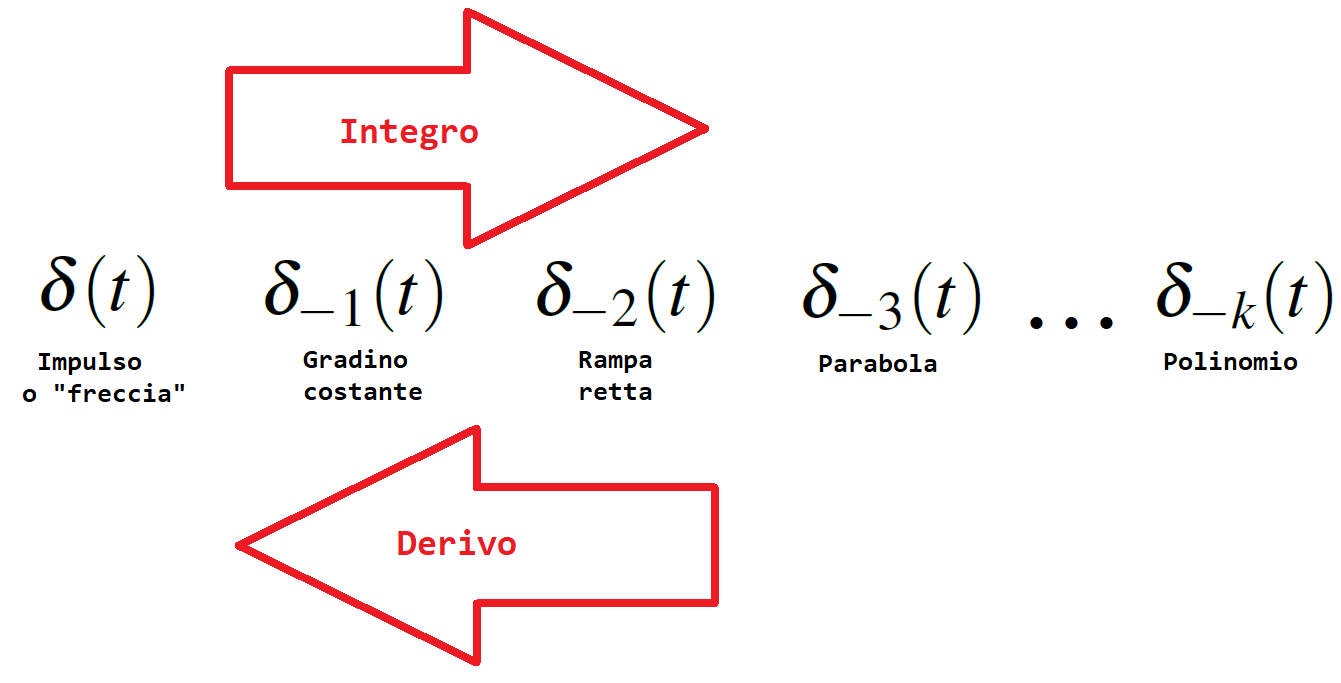
\includegraphics[scale=0.5]{immagini/riassuntoDistribuzioni}
		\caption{ Relazioni fra distribuzioni }
		\label{fig: riassuntoDistribuzioni}
	\end{figure} 

\subsubsection{Delta o impulso di Dirac}
	
	Abbiamo visto fino adesso funzioni generalizzate nel senso delle distribuzioni, cioè il limite di una serie di funzioni.\\
	Definiamo ora l'impulso di Dirac $ \delta(t)$ (sarebbe $ \delta_0 (t)$) come la derivata di $ \delta_{-1} (t)$ dal punto di vista delle distribuzioni (funzioni generealizzate, cioè limiti di successioni di funzioni).\\
	
	\textbf{OSS:} $ \delta_{-1} (t)$ come fuonzione standard non è continua e quindi non derivabile in $ t=0 $ ma nel senso delle distribuzioni si. Vogliamo vedere quindi $ \delta_{-1} (t)$ come il limite di $ \delta_{ \epsilon} (t)$.\\
	
	\begin{figure}[h]
		\centering
		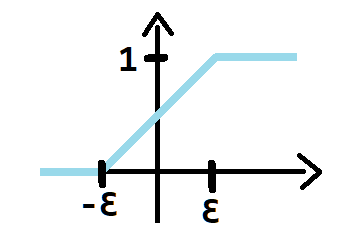
\includegraphics[scale=0.5]{immagini/deltaEpsilon}
		\caption{ $ \delta_{ \epsilon} (t)$ }
		\label{fig: deltaEpsilon}
	\end{figure}
	
	\begin{equation*}
	\delta_{ \epsilon}(t)=
	\begin{cases} 
	0, \mbox{ se } t < - \epsilon \\ 
	\frac{1}{2 \epsilon}t + \frac{1}{2}, \mbox{ se } - \epsilon \leq t < \epsilon\\
	1, \mbox{ se } t \geq \epsilon
	\end{cases} 
	\end{equation*}
	
	\begin{equation*}
	\delta_{-1}(t)= \lim_{ \epsilon \to 0} \delta_{\epsilon}(t)
	\end{equation*}

	Voglio ora una successione con $ n \in \mathbb{N} $ quindi sostituisco $ \epsilon = \frac{1}{n}$.\\
	Ottengo quindi $ \delta_{-1}(t)= \lim_{ n \to \infty} \delta_{\frac{1}{n}}(t) $ (ci sarà utile più avanti).\\
	
	Derivo ora $\delta_{-1}(t)= \lim_{ \epsilon \to 0} \delta_{\epsilon}(t) $: la parte a sinistra è facile da derivare perchè da prima so che $ \delta (t) = \frac{d}{dt} \delta_{-1}(t) $ mentre la parte a destra la dovremo fare per tratti (vedi com'è $ \delta_{\epsilon}(t) $ e lascia stare il limite).\\
	Ci verrà fuori che:
	\begin{equation*}
	\delta(t)= \lim_{ \epsilon \to 0} \frac{1}{2 \epsilon}  \varPi_{\epsilon}(\frac{t}{2 \epsilon})
	\end{equation*}
	
	\begin{figure}[h]
		\centering
		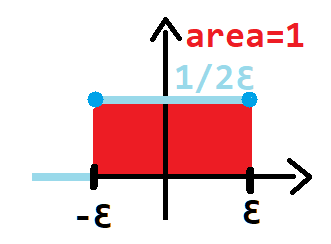
\includegraphics[scale=0.5]{immagini/rettangoloEpsilon}
		\caption{ $ \frac{1}{2 \epsilon}  \varPi_{\epsilon}(\frac{t}{2 \epsilon}) $ }
		\label{fig: rettangoloEpsilon}
	\end{figure}

	\textbf{OSS:} $ \forall \epsilon$, l'area è $\dfrac{1}{2 \epsilon} 2 \epsilon= 1 $ quindi l'area: è indipendente da $ \epsilon$, è costante e non cambia al variare di $ \epsilon $.\\
	
	\textbf{OSS:} per $ \epsilon \rightarrow 0 $ con $ \epsilon > 0 $, ho che $\dfrac{1}{2 \epsilon} \rightarrow \infty $ quindi l'area è sempre 1 ma l'ampiezza tende a $ + \infty $.\\
	
	\textbf{OSS:} $  \int_{ -\infty}^{ \infty} \delta(t)  \, dt = 1   $.\\
	
	\begin{figure}[h]
		\centering
		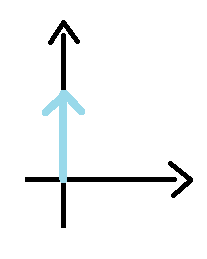
\includegraphics[scale=0.5]{immagini/delta}
		\caption{ Impulso di Dirac }
		\label{fig: delta}
	\end{figure}
	
	\textbf{NB:} può essere definita anche come il limite della seguente successione di funzioni:\\
	\begin{equation*}
	\forall n \in \mathbb{N} f_n(t)=
	\begin{cases} 
	\frac{n}{2}, \mbox{ se } -\frac{1}{n}\leq t \leq \frac{1}{n}\\
	0, \mbox{ altrimenti }
	\end{cases} 
	\end{equation*}
	
\pagebreak

	\begin{figure}[h]
		\centering
		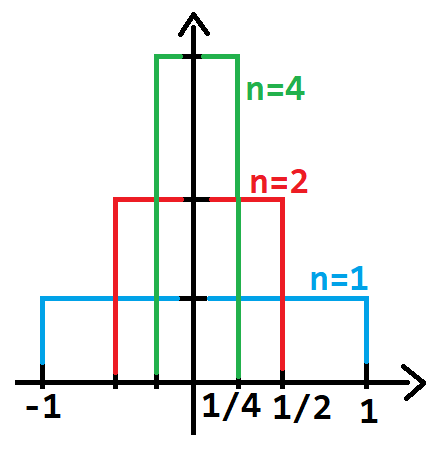
\includegraphics[scale=0.5]{immagini/deltaSuccessione}
		\caption{ $ f_n(t) $ }
		\label{fig: deltaSuccessione}
	\end{figure}

	Il limite quindi sarà:\\
	\begin{equation*}
	\lim_{ n \rightarrow \infty} f_n(t) = \delta(t) 
	\end{equation*}

\subsubsection{Proprietà dell'impulso}

	\textbf{1. } $\forall t \in \mathbb{R} \setminus $ \{ $ 0 $ \} cioè per $ t \neq 0 $ ho $ \delta(t)=0 $. \\
	
	\textbf{2. } (con O intendiamo l'origine)
	
	\begin{equation*}
	\int_{ a}^{ b} \delta( \tau)  \, d\tau =
	\begin{cases} 
	1, \mbox{ se } O \in (a...b)\\
	0, \mbox{ se } O \notin (a...b)
	\end{cases} 
	\end{equation*}
	
	\textbf{3. } Ho che $ \delta(t)=\delta(-t) $, quindi $ \delta(t) $ è pari.\\
	
	\textbf{4. Proprietà del campionamento}\\
	Se $ v(t) $ è continua in $ t_0 $ allora $ \forall t \in \mathbb{R}$:
	\begin{equation*}
	v(t) \delta (t-t_0) = v(t_0) \delta (t-t_0)
	\end{equation*}
	
	%TODO: da questo disegno in poi è tutto misterioso
	\begin{figure}[h]
		\centering
		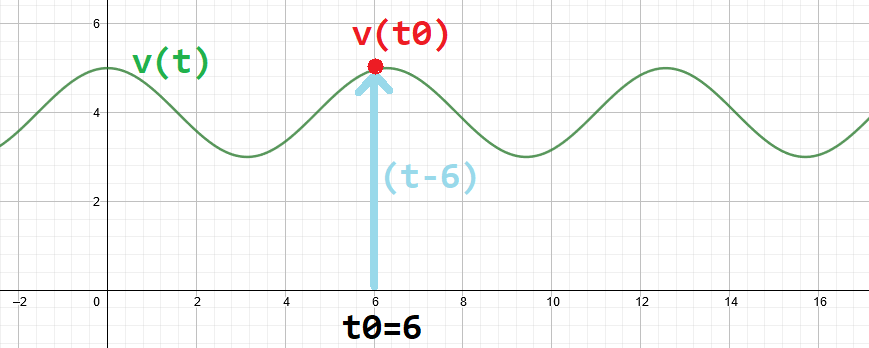
\includegraphics[scale=0.5]{immagini/campionamento}
		\caption{ Proprietà del campionamento }
		\label{fig: campionamento}
	\end{figure}

	\begin{equation*}
	v(t_0) = \int_{ - \infty}^{ \infty} v(t_0) \delta( \tau -t_0)  \, d\tau
	\end{equation*}
	
	\textbf{Conseguenze: }\\
	
	\textbf{1. } Per $ t=0 $ avrò che $ v(t) \delta (t) = v(t_0) \delta (t) $.\\
	
	\textbf{2. } Integriamo $ v(t) \delta (t-t_0) = v(t_0) \delta (t-t_0) $ verrà fuori che:\\
	$ \int_{ - \infty}^{ \infty} v( \tau ) \delta( \tau -t_0)  \, d\tau = \int_{ - \infty}^{ \infty} v( t_0 ) \delta( \tau -t_0)  \, d\tau$\\
	Di questa equazione posso rielaborare la parte destra considerando che $ v(t_0)$ non dipende da $ \tau $ e l'integrale di $ \delta (t-t_0) $ è 1. Quindi viene che:\\
	$ \int_{ - \infty}^{ \infty} v( \tau ) \delta( \tau -t_0)  \, d\tau = v(t_0)$\\
	
	\textbf{ $ \Rightarrow $ Proprietà di riproducibilità dell'impulso }\\
	%TODO: mi sa che qui c'è un errore, guarda bene i tuoi appunti
	Se $ v(t)$ è continua per $ \forall t \in \mathbb{R} $\\
	allora
	\begin{equation*}
	v(t) = \int_{ - \infty}^{ \infty} v( t ) \delta( \tau -t)  \, d \tau
	\end{equation*}
	\textbf{NB:} invece che $ t_0$ ho messo t perchè lo voglio generico avendo v(t) continua.\\
	
	\begin{proof}[Dim]
		Parto con un arteficio (da prendere così come ce l'ha dato il prof): $ v(t)=v(t_0)+( v(t) - v(t_0) )$\\
		Moltiplico da entrambe le parti per $ \delta (t-t_0)$:\\
		$ v(t) \delta (t-t_0) =v(t_0) \delta (t-t_0) +( v(t) - v(t_0) ) \delta (t-t_0) $\\
		Cambio t con $ \tau $ e integro:\\
		$ \int_{ - \infty}^{ \infty} v(\tau) \delta (\tau-t_0) \, d\tau 
		= \int_{ - \infty}^{ \infty} v(t_0) \delta (\tau-t_0) \, d\tau 
		+ \int_{ - \infty}^{ \infty} ( v(\tau) - v(t_0) ) \delta (\tau-t_0)\, d\tau $\\
		Qui devo fare varie considerazioni:\\
		1. Nel secondo integrale $ v(t_0) $ non dipende da $ \tau $ quindi posso portarlo fuori dall'integrale. \\
		2. Sempre nel secondo integrale, l'integrale di $ \delta (\tau-t_0) $ dà 1.\\
		3. Nel terzo integrale:\\
		Se ho $ \tau = t $ allora $ ( v(\tau) - v(t_0) ) = 0 $. \\
		Se ho $ \tau \neq t $ allora $ \delta (\tau-t_0) = 0 $. \\
		Allora il terzo integrale scompare.\\
		Quindi in fine avrò trovato che:\\
		$ \int_{ - \infty}^{ \infty} v(\tau) \delta (\tau-t_0) \, d\tau = v(t_0) $\\
		Questo vale per $ \forall t_0 $ per cui v(t) è continua (rendo quindi $t_0$ generica mettendo al suo posto t).\\ Quindi posso scrivere che:\\
		$ v(t) = \int_{ - \infty}^{ \infty} v(\tau) \delta (\tau-t) \, d\tau$
	\end{proof}

\subsubsection{Impulso centrato in $t_0$ e di area A: $ A \delta (t-t_0)$}

	\begin{figure}[h]
		\centering
		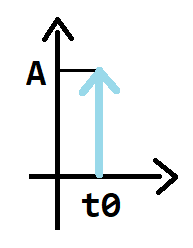
\includegraphics[scale=0.5]{immagini/deltaGenerica}
		\caption{ $ A \delta (t-t_0)$ }
		\label{fig: deltaGenerica}
	\end{figure}

\pagebreak

	\textbf{MATLAB}\\

	\begin{figure}[h]
		\centering
		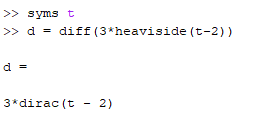
\includegraphics{immagini/comando3}
		\caption{Il comando syms mi crea una variabile t, diff mi fà la derivata di heaviside cioè il gradino. Come risultato ho dirac cioè proprio l'impulso.  }
		\label{fig: comando3}
	\end{figure}

\section{A tempo discreto}

Un segnale a tempo discreto è così definito (useremo k al posto di t per distinguerli):\\
$ v(k): \mathbb{Z} \rightarrow \mathbb{R} $

\subsubsection{Impulso discreto unitario (impulso di Kronecker)}

	\begin{equation*}
	\delta(k)=
	\begin{cases} 
	1, \mbox{ se } k=0 \\
	0, \mbox{ se } k \neq 0
	\end{cases} 
	\end{equation*}

	\begin{figure}[h]
	\centering
	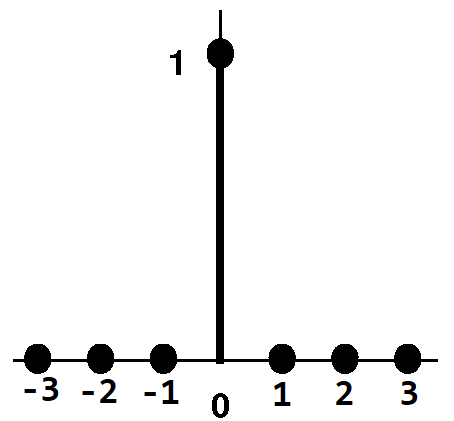
\includegraphics[scale=0.5]{immagini/impulsoDiscreto}
	\caption{ $ \delta(k)$ }
	\label{fig: impulsoDiscreto}
	\end{figure}

\subsubsection{Gradino discreto}

	\begin{equation*}
	\delta_{-1}(k)=
	\begin{cases} 
	1, \mbox{ se } k \geq 0 \\
	0, \mbox{ se } k < 0
	\end{cases} 
	\end{equation*}

\pagebreak
	
	\begin{figure}[h]
		\centering
		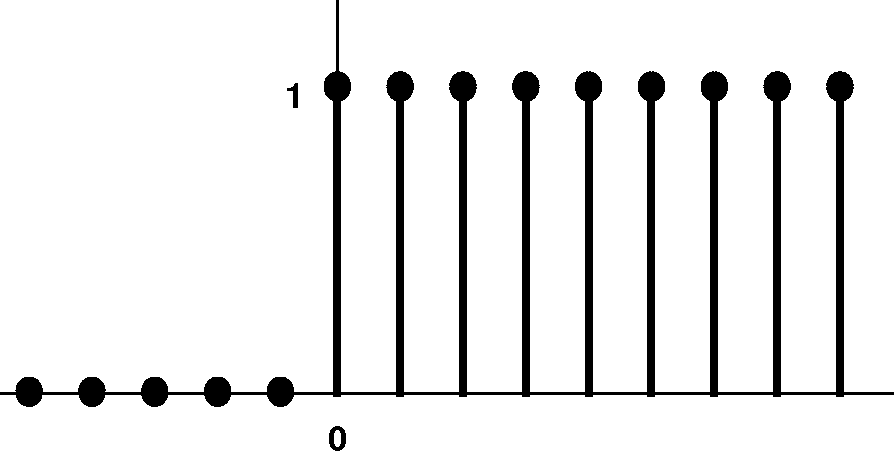
\includegraphics[scale=0.5]{immagini/gradino}
		\caption{ $ \delta_{-1}(k)$ }
		\label{fig: gradino}
	\end{figure}

	\textbf{OSS:}\\
	Se prendo $ k=-1 $, avrò $ \delta_{-1}(-1) = 0 $.\\
	Se prendo $ k=0 $, avrò $ \delta_{-1}(0) = \delta(0) = 1 $.\\
	Se prendo $ k=1 $, avrò $ \delta_{-1}(1) = \delta(0) = 1 $.\\
	
	%TODO: non ho capito
	\begin{equation*}
	\delta_{-1}(k)= \sum_{i=-\infty}^{k} \delta(i)
	\end{equation*}

\subsubsection{Rampa discreta}

	\begin{equation*}
	\delta_{-2}(k)=
	\begin{cases} 
	k, \mbox{ se } k \geq 0 \\
	0, \mbox{ se } k < 0
	\end{cases} 
	\end{equation*}
	
	\begin{figure}[h]
		\centering
		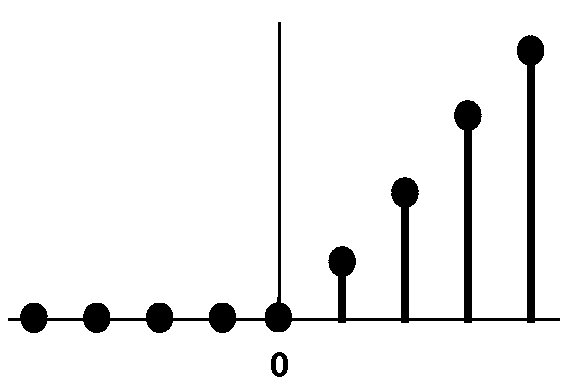
\includegraphics[scale=0.5]{immagini/rampaDiscreta}
		\caption{ $ \delta_{-2}(k)$ }
		\label{fig: rampaDiscreta}
	\end{figure}
	
	\textbf{OSS:}\\
	$ \delta_{-2}(0) = \sum_{i=-\infty}^{-1} \delta_{-1}(i) =0 $\\
	$ \delta_{-2}(1) = \sum_{i=-\infty}^{0} \delta_{-1}(i) = \delta_{-1}(0) $\\
	$ \delta_{-2}(2) = \sum_{i=-\infty}^{1} \delta_{-1}(i) = \delta_{-1}(0) + \delta_{-1}(1) $\\
	
	Si deduce quindi che:\\
	\begin{equation*}
	\delta_{-2}(k)= \sum_{i=-\infty}^{k-1} \delta_{-1}(i)
	\end{equation*}
	
	Ma allora questo significa che:\\
	\begin{equation*}
	\delta_{-2}(k)= \sum_{i=-\infty}^{ \infty} \sum_{j=-\infty}^{k-1} \delta(j)
	\end{equation*}
	
	Se $ k=0 $, allora $ \delta_{-2}(0) =0  $\\
	Se $ k=1 $, allora $ \delta_{-2}(1) = \delta_{-1}(0) = \delta(0) = 1  $\\
	Se $ k=2 $, allora $ \delta_{-2}(2) = \delta_{-1}(0) + \delta_{-1}(1) = \delta(0) + \delta(0) + \delta(1) = 1+1+0=2  $\\
	
	\textbf{Problema del campionamento ma in modo discreto }\\
	
	\begin{figure}[h]
		\centering
		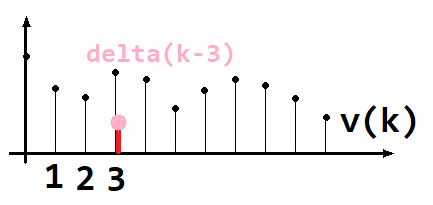
\includegraphics[scale=0.5]{immagini/campionamentoDiscreto}
		\caption{ Segnale a tempo discreto, $\delta(i-3)$ è l'impulso traslato in 3}
		\label{fig: campionamentoDiscreto}
	\end{figure}
	
	Il segnale v(k) ora è discreto (successione, $ k \in \mathbb{Z}$).\\
	Possiamo scrivere il segnale come:\\
	\begin{equation*}
	v(k)= \sum_{i=-\infty}^{ \infty} v(i) \delta(i-k)
	\end{equation*}
	
	In un determinato punto $ k=3$ sarà:\\
	\begin{equation*}
	v(3)= \sum_{i=-\infty}^{ \infty} v(i) \delta(i-3)
	\end{equation*}
	Tutti i termini della sommatoria saranno 0 a parte in 3.\\
	$ ...+0+0+0+ v(3) \delta(3-3)+0+0+0+...= v(3) \delta(0) = v(3)1 = v(3)$

\subsubsection{Successioni esponenziali}

	L'analogo segnale discreto è:
	\begin{equation*}
	v(k)= Ae^{j \phi} \lambda^k
	\end{equation*}
	con $ k \in \mathbb{Z} $, l'ampiezza $ A \in \mathbb{R}_+ $, $ \phi \in \mathbb{R} $ e $ \lambda \in \mathbb{C}$.\\
	
	Ricordiamo che $ \lambda $ essendo un numero complesso posso scriverlo anche come:\\
	 $ \rho ( cos\theta + j sen\theta) = \rho e^{j \theta} $\\
	Il segnale quindi diventerà:\\
	$ v(k)= Ae^{j \theta} \lambda^k = Ae^{j \theta} \rho^{k} e^{j \theta k} = Ae^{j \theta} e^{ (ln(\rho)+j\theta) k} $\\
	\textbf{NB:} nell'ultimo passaggio ho usato $ \rho = e^{ln(\rho)}$.\\
	\textbf{OSS:} v(k) può essere visto come la versione campionata (con periodo di campionamento unitario) del segnale esponenziale continuo.\\
	$ v(t) = Ae^{j \theta} e^{ ut} $ dove $ u=ln( \rho)+j \theta $.\\
	

\subsubsection{Successioni sinusoidali}

	L'analogo segnale discreto è:
	\begin{equation*}
	v(k)= Acos( \theta k + \phi)
	\end{equation*}
	con l'ampiezza $ A>0 $, $ \theta $ è la pulsazione e $ \phi$ la fase.\\
	
	v(k) è periodico se e solo se $ \theta = \frac{2 \pi n}{N}$, dove $n \in \mathbb{N} $, cioè è un multiplo razionale di $ 2 \pi $.\\
	$ N>0 $ è i periodo.\\
	

\subsubsection{Successioni sinusoidali modulate esponenzialmente}

	L'analogo segnale discreto è:
	\begin{equation*}
	v(k)= A \rho^k cos( \theta k + \phi)
	\end{equation*}
	con $ A>0 $, $ \rho>0 $, $ \theta$ e $\phi \in \mathbb{R}$.\\
	
	v(k) non è periodico perchè ho un esponenziale, si dice che v(k) è pseudo-periodico perchè devo comunque guardare la frequenza del campionamento.










